% !TEX root = saveliev_physics_general_course_1.tex
%!TEX TS-program = pdflatex
%!TEX encoding = UTF-8 Unicode

\chapter[PHASE EQUILIBRIA AND TRANSITIONS]{PHASE EQUILIBRIA\\ AND TRANSITIONS}\label{chap:15}
\chaptermark{PHASE EQUILIBRIA AND TRANSITIONS}

\section{Introduction}\label{sec:15_1}

By a phase in thermodynamics is meant a combination of homogeneous parts of a system having identical properties. Let us explain what is meant by this definition using the following examples. A closed vessel contains water and a mixture of air and water vapour above it. Here we have to do with a system consisting of two phases: one is formed by the water, and the other by the mixture of air and water vapour. If we add a few pieces of ice to the water, then all these pieces form a third phase. Different crystalline modifications of a substance are also different phases. For instance, diamond and graphite are different solid phases of carbon.

In definite conditions, different phases of the same substance can be in equilibrium with one another while being in contact. The equilibrium of two phases is possible only within a definite temperature interval, and a quite definite pressure $p$ at which equilibrium is possible corresponds to each value of the temperature $T$. Thus, the equilibrium states of two phases will be depicted in a $p$-$T$ diagram by the line
\begin{equation}\label{eq:15_1}
    p = f(T).
\end{equation}

Three phases of a single substance (solid, liquid, and gaseous, or liquid and two solid phases) can be in equilibrium only at single values of the temperature and pressure which in the $p$-$T$ diagram correspond to what we call the \textbf{triple point}. This point is at the intersection of the equilibrium curves for the phases taken in pairs.

It is proved in thermodynamics, in agreement with experiments, that the equilibrium of more than three phases of the same substance is impossible.

The transition from one phase to another is usually attended by the absorption or liberation of a certain amount of heat called the \textbf{latent heat of transition} or simply the \textbf{heat of transition}. Such transitions are called phase transitions of the first kind. There are also transitions from the crystalline modification to another that are not associated with the absorption or liberation of heat. These transitions are called phase transitions of the second kind\footnote{Phase transitions of the second kind do not exhaust the transitions between different crystalline modifications. They include the transition to a superconductive state performed in the absence of a magnetic field, and also the transition between the two liquid phases of helium called helium-I and helium-II.}. We shall consider only transitions of the first kind.

\section{Evaporation and Condensation}\label{sec:15_2}

Liquids and solids at any temperature contain a certain number of molecules whose energy is sufficient for them to overcome the attraction to other molecules, escape from the surface of the liquid or solid and to pass over into the gaseous phase. The transition of a liquid into the gaseous phase is called \textbf{vaporization} or \textbf{evaporation}, and the transition of a solid into the gaseous phase is called \textbf{sublimation}.

All solids sublime to some extent without any exception. In some substances such as carbon dioxide, sublimation proceeds at an appreciable rate; in other substances, it is so insignificant at ordinary temperatures that it is practically not detected.

In evaporation and sublimation, the fastest molecules leave a body. As a result, the mean energy of the remaining molecules diminishes, and the body cools. To maintain the temperature of an evaporating (or subliming) body at a constant value, heat must continuously be supplied to it. The heat $L$ that must be supplied to a unit mass of a substance to transform it into a vapour at the same temperature which the substance had prior to evaporation is defined as the \textbf{specific heat of vaporization} (or sublimation).

In condensation, the heat for evaporation is returned: the liquid (or solid) formed upon condensation is heated.

Let us consider the setting in of equilibrium between a liquid and its vapour. We shall take a sealed vessel partly filled with a liquid (\fig{15_1}) and assume that initially the substance was completely removed from the space above the liquid. Owing to evaporation, the space above the liquid will become filled with molecules. The molecules that passed into the gaseous phase move chaotically and collide with the surface of the liquid. Some of these collisions will be attended by transition of the molecules into the liquid phase. The number of molecules passing in unit time into the liquid phase is evidently proportional to the number of molecules colliding with its surface. This number, in turn, is proportional to $n\average{v}$ [see \eqn{11_23}], \ie, grows with increasing pressure $p$. Hence, evaporation is accompanied by the reverse process of transition of the molecules from the gaseous to the liquid phase, its intensity growing as the density of the molecules in the space over the liquid increases. When a certain quite definite (for the given temperature) pressure is reached, the number of molecules escaping from the liquid will become equal to that returning to it. Beginning from this moment, the density of the vapour stops changing. Mobile equilibrium sets in between the liquid and its vapour, and it will exist until the volume or the temperature of the system changes. A vapour in equilibrium with its liquid is called \textbf{saturated}. The pressure at which equilibrium is observed is called the \textbf{saturated vapour pressure}.

\begin{figure}[t]
	\begin{center}
		
\includegraphics[scale=0.9]{figures/ch_15/fig_15_1.pdf}
		\caption[]{}
		\label{fig:15_1}
	\end{center}
	\vspace{-0.8cm}
\end{figure}

The number of molecules leaving a liquid in unit time grows very rapidly with the temperature. The number of molecules colliding with the surface of the liquid depends on the temperature to a smaller extent (through $\average{v}$ in proportion to $\sqrt{T}$). Therefore, upon elevation of the temperature, equilibrium between the phases is violated, and during a certain time the stream of molecules travelling in the direction liquid $\to$ vapour will exceed their stream in the direction vapour $\to$ liquid. This continues until the increase in the pressure again leads to the setting in of mobile equilibrium. Thus, the pressure at which mobile equilibrium sets in between a liquid and its vapour, \ie, the saturated vapour pressure, is found to depend on the temperature. The form of this relation is shown in \fig{15_2}. The meaning of the symbols $\ab{T}{cr}$ and $\ab{p}{cr}$ will come to light in \sect{15_4}.

\begin{figure}[t]
	\begin{center}
		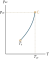
\includegraphics[scale=0.95]{figures/ch_15/fig_15_2.pdf}
		\caption[]{}
		\label{fig:15_2}
	\end{center}
	\vspace{-0.8cm}
\end{figure}

If we increase the volume of the vessel, the vapour pressure will drop, and equilibrium will be violated. As a result, an additional amount of the liquid will transform into a vapour to make the pressure equal to $\ab{p}{sv}$, again. Similarly, reduction of the volume will cause a certain amount of the vapour to transform into a liquid.

Everything said above about equilibrium between a liquid and a gas also holds for a solid-gas system. A definite value of the pressure at which mobile equilibrium sets in between the solid and the gas corresponds to every temperature. For many bodies such as solid metals, this pressure at ordinary temperatures is so small that it cannot be detected by the most sensitive instruments.

\section{Equilibrium Between a Liquid and Its Saturated Vapour}\label{sec:15_3}

Let us consider the compression of a substance at a constant temperature. Assume that the substance is initially gaseous. First, the pressure of the gas will grow with decreasing volume (\fig{15_3}). When the volume $\ab{V}{g}$ is reached, the pressure stops changing, and the substance stops being homogeneous---part of the gas condenses into a liquid. The substance stratifies into two phases: a liquid and a gaseous one. A further reduction of the volume is attended by more and more of the substance passing over into the liquid phase, the transition occurring at a constant pressure $\ab{p}{sv}$ (the saturated vapour pressure). After condensation of the substance terminates (this occurs when the volume $\ab{V}{lq}$ is reached), a further reduction in the volume begins to be attended by a rapid growth of the pressure.

\begin{figure}[t]
	\begin{center}
		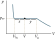
\includegraphics[scale=1]{figures/ch_15/fig_15_3.pdf}
		\caption[]{}
		\label{fig:15_3}
	\end{center}
	\vspace{-0.8cm}
\end{figure}

In \fig{15_3}, $\ab{V}{ab}$ is the volume occupied by the substance in the gaseous state at the pressure $\ab{p}{sv}$ and $\ab{V}{lq}$ is the volume of the substance in the liquid state at the same pressure. At any intermediate value of the volume $V$, part of the substance with the mass $\ab{m}{lq}$ will be in the liquid state, and part with the mass $\ab{m}{v}$ in the vapour state. Let us find the ratio $\ab{m}{lq}/\ab{m}{v}$.

We shall call the volume of a unit mass of a substance its specific volume $V'$. Thus, if the mass of a substance is $m$, then the specific volumes of its saturated vapour and liquid at the pressure $\ab{p}{sv}$ will be
\begin{equation}\label{eq:15_2}
    \ab{V}{v}' = \frac{\ab{V}{g}}{m},\quad \ab{V}{lq}' = \frac{\ab{V}{lq}}{m}.
\end{equation}

\noindent
In the state when the mass of the liquid phase is $\ab{m}{lq}$ and that of the vapour is $\ab{m}{v}$, the liquid will occupy the volume $\ab{V}{lq}'\ab{m}{lq}$, and the saturated vapour, the volume $\ab{V}{v}'\ab{m}{v}$. The sum of these two volumes must equal the volume $V$:
\begin{equation*}
    V = \ab{V}{lq}'\ab{m}{lq} + \ab{V}{v}'\ab{m}{v}.
\end{equation*}

\noindent
Introducing into this equation expressions~\eqref{eq:15_2} for the specific volumes and substituting the $\ab{m}{lq}+\ab{m}{v}$ for the mass $m$, we get
\begin{equation*}
    V = \ab{V}{lq}' \parenthesis{\frac{\ab{m}{lq}}{\ab{m}{lq}+\ab{m}{v}}} + \ab{V}{v}' \parenthesis{\frac{\ab{m}{v}}{\ab{m}{lq}+\ab{m}{v}}}.
\end{equation*}

\noindent
Hence,
\begin{equation}\label{eq:15_3}
    \frac{\ab{m}{lq}}{\ab{m}{v}} = \frac{\ab{V}{g} - V}{V - \ab{V}{lq}} = \frac{y}{x}
\end{equation}

\noindent
(see \fig{15_3}). Thus, the ratio of the masses of the liquid and the saturated vapour in a two-phase state equals the ratio of the lengths into which the point depicting the state divides the horizontal portion of the isotherm.

It must be noted that at temperatures far from the critical one (the critical temperature will be treated in the following section) the difference between the volumes of a liquid and its vapour is much greater than that shown in \fig{15_3}. For example, the specific volume of saturated water vapour at \SI{100}{\degreeCelsius} is $1600$ times that of the specific volume of liquid water at the same temperature.

Thus, a horizontal portion of an isotherm corresponds to the states of equilibrium between a liquid and its saturated vapour in a $p$-$V$ diagram. This result is common for all two-phase states---a horizontal portion corresponds to a two-phase system on an isotherm depicted in the variables $p$ and $V$. The ends of this portion correspond to the volumes $V_1$ and $V_2$ occupied by the substance in the first and second phases. These phases may be a liquid and its saturated vapour, or a liquid and crystals (see \fig{15_4}), or, finally, two crystalline modifications of the same substance. In all cases, an equation similar to~\eqref{eq:15_3} holds:
\begin{equation*}
    \frac{m_1}{m_2} = \frac{V_2 - V}{V - V_1}
\end{equation*}

\noindent
($m_1$ and $m_2$ are the masses of the substance in the first and second
phases).

\section{The Critical State}\label{sec:15_4}

Figure~\ref{fig:15_4} gives isotherms for several values of the temperature. A glance at the figure shows that the horizontal portion of the isotherm diminishes in length with elevation of the temperature, and contracts into a point at the temperature $\ab{T}{cr}$ called the \textbf{critical} one. The difference between the specific volumes diminishes accordingly, and together with it the difference between the densities of the liquid and its saturated vapour. This difference vanishes completely at the critical temperature. Simultaneously, any difference between a liquid and its vapour vanishes. The temperature dependence of the density of a liquid and its saturated vapour is shown in \fig{15_5}.

\begin{figure}[t]
	\begin{minipage}[t]{0.5\linewidth}
		\begin{center}
			
\includegraphics[scale=1]{figures/ch_15/fig_15_4.pdf}
			\caption[]{}
			\label{fig:15_4}
		\end{center}
	\end{minipage}
	\hspace{-0.05cm}
	\begin{minipage}[t]{0.5\linewidth}
		\begin{center}
			
\includegraphics[scale=1]{figures/ch_15/fig_15_5.pdf}
			\caption[]{}
			\label{fig:15_5}
		\end{center}
	\end{minipage}
	\vspace{-0.4cm}
\end{figure}

Point C is the limit which the horizontal portions of the isotherms tend to when the temperature tends to its critical value $\ab{T}{cr}$. It is called the \textbf{critical point}. The state depicted by point C is defined as the \textbf{critical state} of a substance. The volume $\ab{V}{cr}$, pressure $\ab{p}{cr}$, and temperature $\ab{T}{cr}$ corresponding to the critical state are called \textbf{critical quantities}. Point C is a point of inflection for the critical isotherm. A tangent to the isotherm at point C is parallel to the $V$-axis.

It can be seen from \fig{15_4} that the saturated vapour pressure grows with the temperature and reaches the value $\ab{p}{cr}$ at the critical temperature. At temperatures above the critical one, the concept of a saturated vapour loses its meaning. Therefore, the curve showing the temperature dependence of the saturated vapour pressure terminates at the critical point (see \fig{15_2}).

If we draw a line through the extreme points of the horizontal portions of the isotherms (\fig{15_4}), we get a bell-shaped curve confining the region of two-phase states of a substance. At above critical temperatures, a substance is homogeneous at any pressure. At such temperatures, a substance cannot be liquefied, no matter what pressure is applied to it.

The concept of the critical temperature was first introduced in 1860 by the Russian scientist Dmitri Mendeleev (1834-1907). He called it the temperature of absolute boiling of a liquid and considered it as the temperature at which the forces of cohesion between the molecules vanish, and a liquid transforms into a vapour regardless of its pressure and the volume it occupies.

\begin{figure}[t]
	\begin{minipage}[t]{0.5\linewidth}
		\begin{center}
			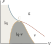
\includegraphics[scale=1]{figures/ch_15/fig_15_6.pdf}
			\caption[]{}
			\label{fig:15_6}
		\end{center}
	\end{minipage}
	\hspace{-0.05cm}
	\begin{minipage}[t]{0.5\linewidth}
		\begin{center}
			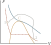
\includegraphics[scale=1]{figures/ch_15/fig_15_7.pdf}
			\caption[]{}
			\label{fig:15_7}
		\end{center}
	\end{minipage}
	\vspace{-0.4cm}
\end{figure}

The bell-shaped curve and the portion of the critical isotherm to the left of point C divide the $p$-$V$ diagram into three regions (\fig{15_6}). The light-shaded area shows the region of homogeneous liquid states of a substance. Under the bell-shaped curve is the region of two-phase states, and, finally, the region to the right of the bell-shaped curve and the upper branch of the critical isotherm is the region of homogeneous gaseous states of a substance. In the latter region, we can earmark the part under the right-hand branch of the critical isotherm and call it the vapour region. Any state in this region differs from the other gaseous states in that upon isothermal compression the substance which was originally in this state is liquefied. The substance in one of the states at a temperature above the critical one cannot be liquefied, no matter what pressure is applied. It is not customary practice to divide the gaseous states into a gas and a vapour.

Having selected a transition process so that it does not intersect a two-phase region (\fig{15_7}), we can ensure a transition from the liquid state to the gaseous one (or vice versa) without separation of the substance into two phases. In this case, the substance will remain homogeneous all the time in the course of the transition process.

\section{Supersaturated Vapour and Superheated Liquid}\label{sec:15_5}

Section~\ref{sec:10_13} gives \eqn{10_62} proposed by van der Waals to describe the state of gases at high densities. Figure~\ref{fig:15_8} depicts van der Waals isotherms, \ie, curves described by \eqn{10_62} for several temperatures. A characteristic of these isotherms is the fact that at temperatures not exceeding the value $\ab{T}{cr}$. the curves have an S-shaped bend in whose region three different values of the volume correspond to a given pressure. Real isotherms (see \fig{15_4}) do not have such a bend, but have a straight horizontal portion instead of it. In \fig{15_9}, a real isotherm and a van der Waals isotherm are superposed on one another. The van der Waals equation describes the path of the isotherm quite well at volumes exceeding $\ab{V}{g}$. At volumes smaller than $\ab{V}{lq}$, the path of a real isotherm also approximately follows the van der Waals equation. Thus, this equation covers not only the gaseous, but also the liquid state of a substance.

\begin{figure}[t]
	\begin{minipage}[t]{0.5\linewidth}
		\begin{center}
			\includegraphics[scale=1]{figures/ch_15/fig_15_8.pdf}
			\caption[]{}
			\label{fig:15_8}
		\end{center}
	\end{minipage}
	\hspace{-0.05cm}
	\begin{minipage}[t]{0.5\linewidth}
		\begin{center}
			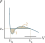
\includegraphics[scale=1]{figures/ch_15/fig_15_9.pdf}
			\caption[]{}
			\label{fig:15_9}
		\end{center}
	\end{minipage}
	\vspace{-0.4cm}
\end{figure}

It can be seen from a comparison of a van der Waals isotherm with a real one that these isotherms approximately coincide on portions corresponding to one-phase states of a substance, but behave absolutely differently in the region of separation into two phases. Instead of the S-shaped bend on the van der Waals isotherm, the real isotherm has a straight horizontal portion in this region which is located so that the shaded areas 1 and 2 enclosed by the bend (\fig{15_9}) are the same.

Separation into two phases is explained by the lack of stability of the homogeneous states corresponding to bend $1$-$2$-$3$-$4$ (\fig{15_10}). The instability of the states between points $2$ and $3$ becomes obvious if we take into account that the derivative $\diffin{p}{V}$ is positive on this part of the bend. Hence, a substance capable of passing consecutively through states $2$-$3$ would have absolutely unnatural properties: an increase in the volume of the gas would be attended by a growth in pressure instead of a reduction in it.

\begin{figure}[t]
	\begin{center}
		\includegraphics[scale=1]{figures/ch_15/fig_15_10.pdf}
		\caption[]{}
		\label{fig:15_10}
	\end{center}
	\vspace{-0.8cm}
\end{figure}

The derivative $\diffin{p}{V}$ is negative on parts $1$-$2$ and $3$-$4$, so that it would seem possible for these portions of the curve to be realized. Indeed, in certain conditions, the states corresponding to these portions can be achieved. True, they are not fully stable: for example, it is sufficient for a dust particle to get into the vapour in state A for the substance to break up into two phases and pass over into
state B (see the transition A $\to$ B shown by the arrow in \fig{15_10}). Such not fully stable states are called \textbf{metastable}. The substance in states $1$-$2$ is called a \textbf{superheated liquid}, and in states $3$-$4$ is called a \textbf{supersaturated vapour}.

At sufficiently low temperatures, the bottom part of the bend in the van der Waals isotherm crosses the $V$-axis and passes into the region of negative pressures (see the bottom isotherm in \fig{15_10}). A substance under a negative pressure is obviously in a state of tension instead of compression. Such states can also be realized in certain conditions. Thus, portion $5$-$6$ on the bottom isotherm corresponds to a \textbf{superheated liquid}, and $6$-$7$ to a \textbf{tensioned liquid}.

Let us consider the conditions in which metastable states can be brought about. We shall begin with a supersaturated vapour. If a vapour contains absolutely no foreign inclusions, its condensation into a liquid cannot begin. For a droplet to form, a great number of molecules must simultaneously approach one another to a distance of the same order as the distances between the molecules in the liquid, and this is absolutely improbable. For condensation to commence, the presence of so-called \textbf{condensation centres} is needed, which capture the molecules flying toward them and transfer them into the condensed phase. Dust particles, liquid droplets, and, especially, charged particles (ions) can be condensation centres.

Thus, if a vapour is thoroughly purified of foreign inclusions and ions, it can be at a pressure exceeding the saturated vapour pressure $\ab{p}{sv}$ at the given temperature. This state will be metastable: it is sufficient for even one condensation centre to appear, and the state of a supersaturated vapour will be violated---the substance will pass over into a two-phase state.

In practice, a supersaturated vapour can be obtained by subjecting one that is not supersaturated to sharp expansion. The rapid expansion occurs without heat exchange with the surroundings and is attended by cooling of the vapour. The point depicting the state of the vapour moves along an adiabat. The latter, as was shown in \sect{10_10}, is steeper than an isotherm. Hence, the vapour can pass over from stable state $1$ corresponding to the temperature $T_1$ (\fig{15_11}) to metastable state $2$ corresponding to the lower temperature $T_2$. Such a process is used in a Wilson cloud chamber---a device intended for observing the traces of charged particles (for example, alpha particles). The air saturated with water or alcohol vapour contained in a Wilson chamber is sharply expanded. The result is cooling of the air, and the vapour becomes supersaturated. A particle flying into the chamber ionizes the molecules along its path. The supersaturated vapour condenses on the ions produced in minute droplets and forms a well visible trace.

Let us consider the conditions for obtaining a superheated liquid. The process of violent vaporization (\ie, boiling) can occur, like the process of condensation, on foreign inclusions, for example, on sand particles or gas bubbles dissolved in the liquid. If a liquid is thoroughly purified of solid inclusions and dissolved gases, then by heating it can be brought into a state with a pressure below $\ab{p}{sv}$ at a given temperature without the liquid boiling. This will be the state of a superheated liquid.

The transition of a liquid from its conventional state to a superheated one is shown in \fig{15_12} (see transition $1$-$2$ shown by the arrow). The state of a superheated liquid is metastable. It is sufficient to throw a sand particle into a superheated liquid for the latter to boil and the substance to pass over into the stable two-phase state (see transition $C$-$D$ in \fig{15_10}).

\begin{figure}[t]
	\begin{minipage}[t]{0.5\linewidth}
		\begin{center}
			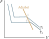
\includegraphics[scale=1]{figures/ch_15/fig_15_11.pdf}
			\caption[]{}
			\label{fig:15_11}
		\end{center}
	\end{minipage}
	\hspace{-0.05cm}
	\begin{minipage}[t]{0.5\linewidth}
		\begin{center}
			\includegraphics[scale=1]{figures/ch_15/fig_15_12.pdf}
			\caption[]{}
			\label{fig:15_12}
		\end{center}
	\end{minipage}
	\vspace{-0.4cm}
\end{figure}

A tensioned liquid, for example, mercury, can be obtained as follows. If we submerge a long glass tube soldered at one end into mercury and, after turning it with its soldered end upward, carefully pull it out from the mercury, then we can get a column of mercury in the tube that considerably exceeds \SI{760}{\milli\metre}. Hence, the mercury will be kept in the tube not by the force of atmospheric pressure, but by the cohesion between its molecules. The mercury in the tube will be in a state of tension, \ie, under a negative pressure.

\section{Melting and Crystallization}\label{sec:15_6}

The transition of a crystalline body to the liquid state takes place at a definite temperature for every substance and requires the expenditure of a certain amount of heat called the \textbf{heat of fusion}.

If a substance originally in the crystalline state receives the same amount of heat every second, its temperature will change with time as shown in \fig{15_13}. First the temperature of the body will constantly grow. When the melting point $\ab{T}{m}$ is reached (point $1$ in \fig{15_13}), the temperature of the body will stop changing although the supply of heat to it is continued. At the same time, the process of melting of the solid body begins, during which new and new portions of the substance transform into a liquid. After the melting process is completed and all of the substance melts (point $2$ in \fig{15_13}), the temperature again begins to rise.

The heating curve of an amorphous body is different (see the dash curve in \fig{15_13}). Upon the uniform supply of heat, the temperature of an amorphous body continuously grows. Amorphous bodies have no definite temperature of transition to the liquid state. This transition occurs continuously, and not in a jump. We can only indicate the temperature interval within which a body softens. The explanation is that liquids and amorphous bodies differ only in the degree of mobility of their molecules---amorphous bodies, as already indicated, are greatly supercooled liquids.

The melting point depends on the pressure. Thus, the transition from a crystalline to a liquid state occurs in quite definite conditions characterized by the values of the pressure and temperature. A curve in a $p$-$T$ diagram called the melting or fusion curve corresponds to a combination of these values. The melting curve is very steep. To change the melting point of ice by one kelvin, for example, the pressure has to be changed by \SI{132}{\atm}.

A point on the melting curve determines the conditions in which the crystalline and the liquid phases can be in equilibrium with each other. Such equilibrium is possible with any ratio between the masses of the liquid and the crystals, \ie, at values of the volume of the system within the limits from $m\ab{V}{s}'$ to $m\ab{V}{lq}'$, where $m$ is the mass of the system, and $\ab{V}{s}'$ and $\ab{V}{lq}'$ are the specific volumes of the solid and the liquid phases. Consequently, in a $p$-$V$ diagram, a portion of a horizontal straight line (\fig{15_14}) corresponds to every point of a melting curve. Since the substance in the states depicted by points on this line has the same temperature, straight line $1$-$2$ in \fig{15_14} is a portion of an isotherm corresponding to two-phase states of the substance (compare with the horizontal portions of the isotherms in \fig{15_14}).

\begin{figure}[t]
	\begin{minipage}[t]{0.5\linewidth}
		\begin{center}
			\includegraphics[scale=1]{figures/ch_15/fig_15_13.pdf}
			\caption[]{}
			\label{fig:15_13}
		\end{center}
	\end{minipage}
	\hspace{-0.05cm}
	\begin{minipage}[t]{0.5\linewidth}
		\begin{center}
			\includegraphics[scale=1]{figures/ch_15/fig_15_14.pdf}
			\caption[]{}
			\label{fig:15_14}
		\end{center}
	\end{minipage}
	\vspace{-0.4cm}
\end{figure}

The process of crystallization that is the reverse of melting proceeds as follows. When a liquid is cooled to a temperature at which the solid and liquid phases can be in equilibrium at the given pressure (\ie, to the same temperature at which melting occurs), the simultaneous growth of minute crystals begins about the so-called \textbf{nuclei} or \textbf{centres of crystallization}. Growing larger and larger, the separate crystals in the long run join one another, forming a polycrystalline solid.

Solid particles suspended in the liquid can be the crystallization centres. A liquid thoroughly purified of such particles can be cooled to below the freezing point without the formation of crystals beginning. The state of such a supercooled liquid is metastable. It is usually sufficient for a dust particle to get into such a liquid for it to break up into a liquid and crystals at the equilibrium temperature. Sometimes upon great supercooling, however, the mobility of the liquid molecules is so insignificant that the metastable state can be preserved for a very long time. The liquid in such cases has a very low fluidity and is an amorphous solid. The process of crystallization is attended by the liberation of the same amount of heat as that absorbed in melting.

\section{The Clapeyron-Clausius Equation}\label{sec:15_7}

We saw in the preceding sections that any two phases of a substance can be in equilibrium only at a definite pressure whose magnitude depends on the temperature. We can obtain the general form of this relation by resorting to the concept of entropy. For this purpose, we shall consider a Carnot cycle for a system consisting of two phases of a given substance in equilibrium.

In a $p$-$V$ diagram, the Carnot cycle for a two-phase system has the form shown in \fig{15_15} (the temperatures of the high temperature and
low temperature reservoirs are assumed to differ by the very small value $\Delta T$). The numbers $1$ and $2$ denote the extreme points of the horizontal portion of the isotherm of temperature $T$. States $1$ and $2$ are one-phase ones. All the intermediate points on $1$-$2$, depict two-phase states differing from each other in the distribution of the mass of the substance between the first and the second phases.

\begin{figure}[t]
	\begin{center}
		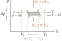
\includegraphics[scale=1]{figures/ch_15/fig_15_15.pdf}
		\caption[]{}
		\label{fig:15_15}
	\end{center}
	\vspace{-0.8cm}
\end{figure}

The isothermal process A $\to$ B is attended by a phase transition of a certain mass $m$ of the substance. The volume of the substance receives an increment of $m(V_2'-V_1')$, where $V_1'$ and $V_2'$ are the specific volumes of the first and second phases. For such a transition to occur, the heat $Q_1$ equal to $mL_{12}$ must be supplied to the substance ($L_{12}$ is the specific heat absorbed in the transition from state $1$ to state $2$ at the temperature $T$). The heat $Q_1$ is the heat which the system receives in the course of the cycle from the high temperature reservoir. The heat is given up to the low temperature reservoir in the course of the isothermal process C $\to$ D.
The heat given up amounts to $Q_2'=m'L_{12}'$, where $L_{12}'$ is the heat of transition $1$-$2$ at the temperature $T-\Delta T$, and $m'$ is the mass of the substance experiencing a phase transition in the course of the process C $\to$ D. This value differs somewhat from $m$ because a certain mass of the substance undergoes phase transitions in the course of adiabatic processes.

On ihe isothermal portion A-B, the entropy of the system receives the increment $\Delta S_1$ equal to $Q_1/T$. On the isothermal portion C-D, the increment of the entropy is $\Delta S_2=-Q_2'(T-\Delta T)$. The entropy does not change in the course of the adiabatic processes B-C and D-A. The total increment of the entropy during a cycle is zero. Hence,
\begin{equation*}
    \Delta S_1 + \Delta S_2 = \frac{Q_1}{T} - \parenthesis{\frac{Q_2'}{T-\Delta T}} = 0
\end{equation*}

\noindent
whence
\begin{equation}\label{eq:15_4}
    \parenthesis{Q_1 - Q_2'}T = Q_1 \Delta T.
\end{equation}

According to \eqn{12_3}, $Q_1-Q_2'$ equals the work done during a cycle. This work can be found by calculating the area of the cycle. Approximately, this area can be considered equal to $m(V_2'-V_1')\Delta p$ (see \fig{15_15}). We thus arrive at the relation
\begin{equation}\label{eq:15_5}
    Q_1 - Q_2' = m\parenthesis{(V_2'-V_1')}\Delta p.
\end{equation}

\noindent
In the limit when $\Delta p$ tends to zero (for which it is necessary that $\Delta T$ also tend to zero), expression~\eqref{eq:15_5} transforms into a strict equality.

Let us substitute expression~\eqref{eq:15_5} in \eqn{15_4} for $Q_1-Q_2'$, and also $mL_{12}$ for $Q_1$. As a result, we get
\begin{equation*}
    m\parenthesis{V_2'-V_1'} T \Delta T. \approx mL_{12} \Delta T.
\end{equation*}

\noindent
Hence,
\begin{equation*}
    \frac{\Delta p}{\Delta T} \approx \frac{L_{12}}{\parenthesis{V_2'-V_1'}}.
\end{equation*}

\noindent
Finally, performing the limit transition $\Delta T\to 0$, we arrive at the strict equation
\begin{equation}\label{eq:15_6}
    \diff{p}{T} = \frac{L_{12}}{\parenthesis{V_2'-V_1'}}.
\end{equation}

\noindent
This expression is called the \textbf{Clapeyron-Clausius} equation. It relates the temperature derivative of the equilibrium pressure to the heat of transition, the temperature, and the difference between the specific volumes of the phases in equilibrium.

According to \eqn{15_6}, the sign of the derivative $\diffin{p}{T}$ depends on what change in the volume---an increase or a reduction---attends a phase transition occurring with the absorption of heat. In the evaporation of a liquid or a solid, the volume always grows, therefore $\diffin{p}{T}$ for a vaporization curve, and also for a sublimation one, can only be positive: elevation of the temperature leads to an increase in the equilibrium pressure.

The volume grows, as a rule, in melting, so that $\diffin{p}{T}>0$: an increase in the pressure raises the melting point. For some substances including water, however, the volume of the liquid phase is less than that of the solid phase $(V_2'-V_1')$\footnote{The volume of water is known to increase when it freezes. For this reason, ice has a smaller density than water.}. In this case, $\diffin{p}{T}<0$---an increase in the pressure is attended by lowering of the melting point. We can melt ice by applying a high pressure to it without raising its temperature above \SI{0}{\degreeCelsius}.

The temperature of transition from one crystalline modification to another will rise or lower with increasing pressure depending on which of the solid phases has a greater specific volume.

\section{Triple Point. Phase Diagram}\label{sec:15_8}

Let us take a substance in the form of a liquid and its saturated vapour in equilibrium with it and withdraw heat from it without changing the volume. This process will be attended by lowering of the temperature of the substance and a corresponding reduction in the pressure. Therefore, the point depicting the state of the substance in a $p$-$T$ diagram will move downward along the vaporization curve (\fig{15_16}). This will continue until the freezing point of the substance is reached corresponding to the equilibrium pressure value. Let us denote this temperature by $\ab{T}{tr}$. The temperature and the pressure remain constant all the time the freezing process goes on. The heat removed during this process is the heat liberated in freezing (crystallization).

\begin{figure}[t]
	\begin{center}
		\includegraphics[scale=1]{figures/ch_15/fig_15_16.pdf}
		\caption[]{}
		\label{fig:15_16}
	\end{center}
	\vspace{-0.8cm}
\end{figure}

The temperature $\ab{T}{tr}$ and the equilibrium pressure $\ab{p}{tr}$ corresponding to it are the only values of the temperature and pressure at which three phases of a substance ---the solid, liquid, and gaseous
ones---can be in equilibrium. The corresponding point in a $p$-$T$ diagram is called a \textbf{triple point}. Thus, a triple point determines the conditions in which three phases of a substance can be in equilibrium simultaneously.

Upon completion of the freezing process, the solid and gaseous phases will be in equilibrium. If we continue to remove heat from the substance, the temperature will again begin to lower. The pressure of the vapour in equilibrium with the crystalline phase will decrease accordingly. The point depicting the state of the substance will move downward along the sublimation curve.

The temperature of a triple point is the temperature at which a substance melts when it is under the pressure $\ab{p}{tr}$. At other pressures, the melting point will be different. The relation between the pressure and the melting point will be depicted by the melting curve beginning at the triple point. Thus, a triple point is on the intersection of three curves determining the conditions of equilibrium of two phases: solid and liquid, liquid and gaseous, and, finally, solid and gaseous.

Depending on the relation between the specific volumes of the solid and liquid phases, the melting curve is directed either as shown in \fig{15_16} ($\diffin{p}{T}>0$) or as shown in \fig{15_17} ($\diffin{p}{T}<0$).

The melting, vaporization, and sublimation curves divide the coordinate plane into three regions. To the left of the sublimation and melting curves is the region of the solid phase, between the melting and vaporization curves is the region of liquid states, and, finally, to the right of the vaporization and sublimation curves is the region of gaseous states of the relevant substance. Any point in one of these regions depicts the corresponding one-phase state of the substance (we always have in view only equilibrium states, \ie, states in which a substance can be as long as desired in unchanging external conditions). A point on one of the curves separating the regions depicts a state of equilibrium of the two relevant phases of the substance. The triple point depicts the state of equilibrium of all three phases. Thus, each point in the diagram depicts a definite equilibrium state of the substance. Such a diagram is called a \textbf{phase diagram}.

The phase diagram is more complicated for a substance having several crystalline modifications. Figure~\ref{fig:15_18} shows a diagram for the case when the number of different crystalline modifications is two. There are two triple points in this case. The liquid, gas, and the first crystalline modification of the substance are in equilibrium at point $\ab{T}{r}$, while the liquid and both crystalline modifications are in equilibrium at point $\ab{T}{r}'$.

\begin{figure}[t]
	\begin{minipage}[t]{0.5\linewidth}
		\begin{center}
			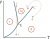
\includegraphics[scale=1]{figures/ch_15/fig_15_17.pdf}
			\caption[]{}
			\label{fig:15_17}
		\end{center}
	\end{minipage}
	\hspace{-0.05cm}
	\begin{minipage}[t]{0.5\linewidth}
		\begin{center}
			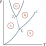
\includegraphics[scale=1]{figures/ch_15/fig_15_18.pdf}
			\caption[]{}
			\label{fig:15_18}
		\end{center}
	\end{minipage}
	\vspace{-0.4cm}
\end{figure}

A phase diagram for each particular substance is plotted on the basis of experimental data. Knowing the phase diagram, we can predict the state in which a substance will be in various conditions (at various values of $p$ and $T$), and also the transformations which the substance will undergo in different processes.

The following examples will explain this. If we take a substance in the state corresponding to point $1$ (see \fig{15_16}) and subject it to isobaric heating, then the substance will pass through the sequence of states shown by the dash straight line $1$-$2$, namely, crystals-liquid-
gas. If we take the same substance in the state depicted by point $3$ and also subject it to isobaric heating, then the sequence of states (dash line $3$-$4$) will be different, namely, the crystals transform directly into a gas without passing through the liquid phase.

It can be seen from the phase diagram that the liquid phase can exist in an equilibrium state only at pressures not lower than that of the triple point (the same relates to the solid phase II in \fig{15_18}). At pressures below $\ab{p}{tr}$ only supercooled liquids are observed. The triple point of most ordinary substances is considerably lower than atmospheric pressure. Hence, the transition of these substances from the solid state to the gaseous one occurs through the intermediate liquid phase. For instance, a pressure of \SI{4.58}{\mmHg} and a temperature of \SI{0.0075}{\degreeCelsius} correspond to the triple point of water. For carbon dioxide, the pressure at the triple point is \SI{5.11}{\atm} (the temperature of the triple point is \SI{-56.6}{\degreeCelsius}). Therefore at atmospheric pressure, carbon dioxide can exist only in the solid and the gaseous states. Solid carbon dioxide (dry ice) transforms directly into a gas. The sublimation point of carbon dioxide at atmospheric pressure is \SI{-78}{\degreeCelsius}.

If the specific volume of crystals exceeds the specific volume of the liquid phase, then the behaviour of the relevant substance in some processes may be quite peculiar. Let us take, for example, such a substance in the state depicted by point $1$ (see \fig{15_17}), and subject it to isothermal compression. The pressure grows in this case, and the process is depicted in the diagram by a vertical straight line (see dash line $1$-$2$). In the course of the process, the substance passes through the following sequence of states: gas-crystals-liquid. Such a sequence is evidently observed at temperatures below that of the triple point.

In concluding, we shall note another feature of a phase diagram. The vaporization curve terminates at the critical point C. Hence, a transition from the region of liquid states to that of gaseous states is possible around the critical point without intersecting the vaporization curve (see transition $3$-$4$ in \fig{15_17} depicted by the dash curve). Figure~\ref{fig:15_11} shows how such a transition looks in a $p$-$V$ diagram. In this case, the transition from the liquid state to the gaseous one (and vice versa) is performed continuously through a sequence of one-phase states. It must be noted that the entire horizontal portion of the relevant isotherm in \fig{15_11} corresponds to the point with the coordinate $T$ taken on the vaporization curve.

The continuous transition between the liquid and the gaseous states is possible because the difference between them is more of a quantitative than of a qualitative nature. In particular, anisotropy is absent in both these states. A continuous transition from the crystalline state to the liquid or gaseous one is impossible because we know that the crystalline state is featured by anisotropy. A transition from a state with anisotropy to one without it can be performed, however, only in a jump. Anisotropy cannot be present only partly either it is present or it is absent, and there is no third possibility. This is why the sublimation and the melting curves cannot terminate at the critical point like the vaporization curve does. The sublimation curve terminates at the point $p=0$ and $T=0$, and the melting curve extends to infinity.

In exactly the same way, a continuous transition from one crystalline modification to another is impossible. Different crystalline modifications of a substance differ in their inherent elements of symmetry. Since a symmetry element may only be either present or absent, the transition from one solid phase to another is possible only in a jump. For this reason, the equilibrium curve of two solid phases, like the melting curve, extends to infinity.
